\documentclass[a4paper,11pt]{exam}
%\printanswers % pour imprimer les réponses (corrigé)
\noprintanswers % Pour ne pas imprimer les réponses (énoncé)
\addpoints % Pour compter les points
% \noaddpoints % pour ne pas compter les points
%\qformat{\textbf{\thequestion ) } }
%\qformat{\textbf{\thequestion )} (\thepoints) \\} % Pour définir le style des questions (facultatif)
\usepackage{color} % définit une nouvelle couleur
\shadedsolutions % définit le style des réponses
% \framedsolutions % définit le style des réponses
\definecolor{SolutionColor}{rgb}{0.8,0.9,1} % bleu ciel
\renewcommand{\solutiontitle}{\noindent\textbf{Solution:}\par\noindent} % Définit le titre des solutions




\makeatletter

\def\maketitle{{\centering%
	\par{\huge\textbf{\@title}}%
	\par{\@date}%
	\par}}

\makeatother

\lhead{NOM Pr\'enom :}
\rhead{\textbf{Les r\'eponses doivent \^etre justifi\'ees}}
\cfoot{\thepage / \pageref{LastPage}}


%\usepackage{../../pas-math}
%\usepackage{../../moncours}


%\usepackage{pas-cours}
%-------------------------------------------------------------------------------
%          -Packages nécessaires pour écrire en Français et en UTF8-
%-------------------------------------------------------------------------------
\usepackage[utf8]{inputenc}
\usepackage[frenchb]{babel}
\usepackage[T1]{fontenc}
\usepackage{lmodern}
\usepackage{textcomp}



%-------------------------------------------------------------------------------

%-------------------------------------------------------------------------------
%                          -Outils de mise en forme-
%-------------------------------------------------------------------------------
\usepackage{hyperref}
\hypersetup{pdfstartview=XYZ}
%\usepackage{enumerate}
\usepackage{graphicx}
\usepackage{multicol}
\usepackage{tabularx}
\usepackage{multirow}


\usepackage{anysize} %%pour pouvoir mettre les marges qu'on veut
%\marginsize{2.5cm}{2.5cm}{2.5cm}{2.5cm}

\usepackage{indentfirst} %%pour que les premier paragraphes soient aussi indentés
\usepackage{verbatim}
\usepackage{enumitem}
\usepackage[usenames,dvipsnames,svgnames,table]{xcolor}

\usepackage{variations}

%-------------------------------------------------------------------------------


%-------------------------------------------------------------------------------
%                  -Nécessaires pour écrire des mathématiques-
%-------------------------------------------------------------------------------
\usepackage{amsfonts}
\usepackage{amssymb}
\usepackage{amsmath}
\usepackage{amsthm}
\usepackage{tikz}
\usepackage{xlop}
%-------------------------------------------------------------------------------



%-------------------------------------------------------------------------------


%-------------------------------------------------------------------------------
%                    - Mise en forme avancée
%-------------------------------------------------------------------------------

\usepackage{ifthen}
\usepackage{ifmtarg}


\newcommand{\ifTrue}[2]{\ifthenelse{\equal{#1}{true}}{#2}{$\qquad \qquad$}}

%-------------------------------------------------------------------------------

%-------------------------------------------------------------------------------
%                     -Mise en forme d'exercices-
%-------------------------------------------------------------------------------
%\newtheoremstyle{exostyle}
%{\topsep}% espace avant
%{\topsep}% espace apres
%{}% Police utilisee par le style de thm
%{}% Indentation (vide = aucune, \parindent = indentation paragraphe)
%{\bfseries}% Police du titre de thm
%{.}% Signe de ponctuation apres le titre du thm
%{ }% Espace apres le titre du thm (\newline = linebreak)
%{\thmname{#1}\thmnumber{ #2}\thmnote{. \normalfont{\textit{#3}}}}% composants du titre du thm : \thmname = nom du thm, \thmnumber = numéro du thm, \thmnote = sous-titre du thm

%\theoremstyle{exostyle}
%\newtheorem{exercice}{Exercice}
%
%\newenvironment{questions}{
%\begin{enumerate}[\hspace{12pt}\bfseries\itshape a.]}{\end{enumerate}
%} %mettre un 1 à la place du a si on veut des numéros au lieu de lettres pour les questions 
%-------------------------------------------------------------------------------

%-------------------------------------------------------------------------------
%                    - Mise en forme de tableaux -
%-------------------------------------------------------------------------------

\renewcommand{\arraystretch}{1.7}

\setlength{\tabcolsep}{1.2cm}

%-------------------------------------------------------------------------------



%-------------------------------------------------------------------------------
%                    - Racourcis d'écriture -
%-------------------------------------------------------------------------------

% Angles orientés (couples de vecteurs)
\newcommand{\aopp}[2]{(\vec{#1}, \vec{#2})} %Les deuc vecteurs sont positifs
\newcommand{\aopn}[2]{(\vec{#1}, -\vec{#2})} %Le second vecteur est négatif
\newcommand{\aonp}[2]{(-\vec{#1}, \vec{#2})} %Le premier vecteur est négatif
\newcommand{\aonn}[2]{(-\vec{#1}, -\vec{#2})} %Les deux vecteurs sont négatifs

%Ensembles mathématiques
\newcommand{\naturels}{\mathbb{N}} %Nombres naturels
\newcommand{\relatifs}{\mathbb{Z}} %Nombres relatifs
\newcommand{\rationnels}{\mathbb{Q}} %Nombres rationnels
\newcommand{\reels}{\mathbb{R}} %Nombres réels
\newcommand{\complexes}{\mathbb{C}} %Nombres complexes


%Intégration des parenthèses aux cosinus
\newcommand{\cosP}[1]{\cos\left(#1\right)}
\newcommand{\sinP}[1]{\sin\left(#1\right)}


%Probas stats
\newcommand{\stat}{statistique}
\newcommand{\stats}{statistiques}
%-------------------------------------------------------------------------------

%-------------------------------------------------------------------------------
%                    - Mise en page -
%-------------------------------------------------------------------------------

\newcommand{\twoCol}[1]{\begin{multicols}{2}#1\end{multicols}}


\setenumerate[1]{font=\bfseries,label=\textit{\alph*})}
\setenumerate[2]{font=\bfseries,label=\arabic*)}


%-------------------------------------------------------------------------------
%                    - Elements cours -
%-------------------------------------------------------------------------------





%\usepackage{fullpage}
\author{\ }
\date{7 octobre 2021}
\title{$5^e $ : DS num\'ero 1}

\graphicspath{{./img/}}

\begin{document}
%	\usepackage{fancyhdr}
%	
%	\pagestyle{fancy}
%	\fancyhf{}
	%\rhead{Share\LaTeX}

	\maketitle
	
\begin{center}
	\textbf{Calculatrice interdite}
\end{center}

\begin{small}
	\begin{center}
		\begin{tabular}{|@{\ }l@{\ }|@{\ }c@{\ }|@{\ }c@{\ }|@{\ }c@{\ }|@{\ }c@{\ }|}
			\hline
			\textbf{Compétence} & \textbf{MI} & \textbf{MF} & \textbf{MS} & \textbf{TBM} \\
			\hline
			\textbf{Calculer} (Calculer avec des nombres décimaux. ) &  \ \ & \ \ & \ \ & \ \  \\
			\hline	
			\textbf{Calculer} (Calculer une expression numérique) &  \ \ & \ \ & \ \ & \ \  \\
			\hline	
			\textbf{Modéliser} (Traduire une situation réelle en langage mathématique) (Ex 4)& \ \ & \ \ &  \ \  & \ \ \\
			\hline
%			\textbf{Modéliser} ( Résolution de problèmes de la vie courante. ) &  \ \ & \ \ & \ \ & \ \  \\
%			\hline
		\end{tabular}
	\end{center}
\end{small}	

	
	
	

%\newpage

%\subsection{Definition}

\begin{mydef}
	
	\iftoggle{eleve}{%
		Effectuer la \hrulefill 
		
		\vspace*{0.2cm}
		\hrulefill 
		
		\vspace*{0.2cm}
		\hrulefill 
		
		
		\vspace*{0.2cm}
		\hrulefill 
		
		
		\vspace*{0.2cm}
		\hrulefill 
		
		
		\vspace*{0.2cm}
		\hrulefill 
	}{%
		Effectuer la \kw{division euclidienne} d’un nombre entier, appelé \kw{dividende}, par un nombre entier, différent de zéro, appelé \kw{diviseur}, c’est trouver deux autres nombres entiers, le \kw{quotient} et le \kw{reste}, tels que : 
		
		\begin{equation*}
			diviseur \times quotient + reste = dividende	
		\end{equation*}
	}
	

	
\end{mydef}


\iftoggle{eleve}{%
	\begin{center}
		$\begin{array}{c|c}
			 &  \hspace*{2cm} \\
			\cline{2-2}
			&  \\
			 & \\
		\end{array}$
	\end{center}
}{%
	\begin{center}
		$\begin{array}{c|c}
			Dividende & Diviseur \\
			\cline{2-2}
			& Quotient \\
			Reste & \\
		\end{array}$
	\end{center}
}


%\begin{mywarning}
%	On ne peut pas diviser par 0.
%\end{mywarning}

%\subsection{Technique de division}

%\begin{mymeth}
%\vspace*{-1cm}	

%\begin{mymethname}{Technique de division}
%\begin{multicols}{2}
%	\begin{center}
%%		$\begin{array}{rc|c}
%%		731 & & 34 \\
%%		\cline{3-3}
%%		51& & 21 \\
%%		17 & & \\
%%		\end{array}$
%		\opidiv{731}{34}
%	\end{center}
%
%Conclusion : $34 \times 21 + 17 = 731$
%\end{multicols}
%
%
%Le diviseur 34 a deux chiffres, on commence la division avec les deux premiers chiffres du dividende $73 > 34 $; 
%combien de fois 34 dans 73 : 2 fois ; on soustrait $2 \times 34$ à 73.
%
%On abaisse le 1. 
%Combien de fois 34 dans 51 : 1 fois ; 
%on soustrait $1 \times 34$ à 51 ; $17 < 34$ ; on a fini.\\
%
%
%\textbf{\underline{Vérification:}}\\
%Il existe un moyen pour vérifier si une division euclidienne est juste. 
%Pour cela, on multiplie le quotient par le diviseur, puis on ajoute le reste. 
%Si le résultat obtenu est égal au dividende, la division est juste.
%\end{mymethname}


\begin{myexs}
	Poser et vérifier les divisions euclidiennes suivantes :  $653 \div 7$ et $73 \div 5$
	
	\vspace*{4cm} 
\end{myexs}

%\begin{mypb}
%	Dans une classe de 26 élèves, on forme des équipes de volley-ball (6 joueurs par équipe).
%	
%	\begin{enumerate}
%		\item Combien d’équipes forme-t-on ?
%		\item Combien y-a-t-il de remplaçants ?	
%	\end{enumerate}
%
%\vspace*{5cm} 	
%\end{mypb}

\section{Division décimale}


\begin{questions}
	\question Poser et calculer la valeur exacte des quotients suivants :
	
	\begin{parts}
		\begin{multicols}{3}
			\part $\num{4.50} \div 9$
			\part $\num{4.20} \div 4$
			\part $\num{31.40} \div 10$
		\end{multicols}
	\end{parts} 
	
	\question Répondre par une phrase aux questions ci-dessous :
	
	\begin{parts}
		\part Quatre ampoules sont vendues \num{4.20} €. Quel est le prix d'une ampoule ?
		
		\part Dix mètres de câble sont vendus \num{31.40} €. Quel est le prix d'un mètre de câble ?
		
		\part Neuf feutres identiques coûtent \num{4.50} €. Quel est le prix de chaque feutre ?
	\end{parts}
	 
	
	
\end{questions}


\section{Calculer}


\begin{questions}
	\question Calculer les expressions suivantes en détaillant tous les calculs :
	
	\begin{enumerate}
		\item $A = 62 - 30 - 7 + 20$
		
		\item $B = (50 - (13 + 1) \times 2) - 6$
		
		\item $C= 225 - ((15 + 7) \times 10 - 2)$
		
		\item $D= (10 \times \num{3.2} - (79 - 71)) \div 6$
	\end{enumerate}
	
	
	\begin{solution}
		
		\begin{multicols}{2}
			
			\begin{eqnarray*}
				A &=& 62 - 30 - 7 + 20 \\
				A &=& 32 - 7 + 20 \\
				A &=& 25 + 20 \\
				A &=& 45
			\end{eqnarray*}
			
			\begin{eqnarray*}
				B &=& (50 - (13 + 1) \times 2) - 6 \\
				B &=& (50 - 14 \times 2) - 6  \\
				B &=& (50 - 28) - 6  \\
				B &=& 22 - 6  \\
				B &=& 16
			\end{eqnarray*}
			
			\begin{eqnarray*}
				C &=& 225 - ((15 + 7) \times 10 - 2)\\
				C &=& 225 - (22 \times 10 - 2) \\
				C &=& 225 - (220 - 2) \\
				C &=& 225 - 218  \\
				C &=& 7
			\end{eqnarray*}
			
			\begin{eqnarray*}
				D &=& (10 \times \num{3.2} - (79 - 71)) \div 6\\
				D &=& (10 \times \num{3.2} - 8) \div 6 \\
				D &=& (32 - 8) \div 6 \\
				D &=& 24 \div 6  \\
				D &=& 4
			\end{eqnarray*}
		\end{multicols}
	\end{solution}
	
	\question Placer des parenthèses pour que l'égalité soit vraie :
	
	s (Répondre directement sur cette feuille) 
	
	\begin{parts}
		\part $ 62 - 30 - 7 + 20 = 59$
		\begin{solution}
			\begin{eqnarray*}
				A &=& 62 - (30 - 7) + 20 \\
				A &=& 62 - 23 + 20 \\
				A &=& 39 + 20 \\
				A &=& 59
			\end{eqnarray*}
		\end{solution}
	
		\part $ 62 - 30 - 7 + 20 = 19$
		\begin{solution}
			\begin{eqnarray*}
				A &=& 62 - (30 - 7 + 20) \\
				A &=& 62 - (23 + 20) \\
				A &=& 62 - 43\\
				A &=& 19
			\end{eqnarray*}
		\end{solution}
	\end{parts}
	 
	
	
	
	
\end{questions}


\newpage

\section{Problèmes}

Pour chaque problème, écrire une expression qui permet de trouver la réponse puis le résoudre en concluant par une phrase.

\begin{questions}
	\question Chloé achète trois livres à \num{5.20} € l'unité et un CD à \num{19.80} €. Elle a payé avec un billet de 50 €. 
	
	Quelle somme lui a-t-on rendue à la caisse ?
	
	\begin{solution}
		\begin{align*}
			A &= 50 - (3 \times \num{5.20} + \num{19.80}) \\
			A &= 50 - (\num{15.60} + \num{19.80}) \\
			A &= 50 - \num{35.40} \\
			A &= \num{14.60}
		\end{align*}
		
		A la caisse, on lui a rendu \num{14.60} €.
	\end{solution}
	
	\question Pour récompenser les vainqueurs du cross du collège, le F.S.E. a acheté 8 coupes à 24 € l'unité et 16 médailles à \num{4.20} € l'unité.
	
	Quelle est la dépense totale du F.S.E. ?
	
	\begin{solution}
		\begin{align*}
			B &= 8 \times 24 + 16 \times \num{4.20} \\
			B &= 192 + \num{67.20} \\
			B &= \num{259.20}
		\end{align*}
		
		Le F.S.E. a dépensé \num{259.20} €.
	\end{solution}
	\question Daniel a gagné \num{4630} € aux courses. Il décide de donner 400 € à l'association du Téléthon, de conserver la moitié du reste pour se payer un voyage, puis de distribuer la somme restante en parts égales à ses cinq petits enfants.
	
	Quelle somme reçoit chacun de ses petits enfants ?
	
	\begin{solution}
		\begin{align*}
			C &= ((4630 - 400) \div 2) \div 3 \\
			C &= (4230 \div 2) \div 5 \\
			C &= 2115 \div 5 \\
			C &= 423 
		\end{align*}
		
		Chacun des petits enfants recevra 423 €.
	\end{solution}
	
	
	\question Hassan a économisé \num{84.70} €. Il s'achète une raquette de tennis à \num{49.50} € et offre la moitié de la somme restante à son jeune frère. 
	
	Quelle somme lui reste-t-il ?
	
	\begin{solution}
		\begin{align*}
			D &= (\num{84.70} - \num{49.50}) \div 2 \\
			D &= \num{35.2} \div 2 \\
			D &= \num{17.6} 
		\end{align*}
		
		Il lui reste \num{17.6} €.
	\end{solution}
	
	\question Emma a acheté trois livres identiques et a payé 36 € en tout. Vincent qui avait 150 €, achète un de ces livres. 
	
	Quelle somme reste-t-il à Vincent ?
	
	\begin{solution}
		\begin{align*}
			E &= 150 - (36 \div 3) \\
			E &= 150 - 12 \\
			E &= 138
		\end{align*}
		
		
		Il reste 138 € à Vincent.
		
	\end{solution}
	
	%	\question[2] Théo doit lire un livre de 150 pages. Le lundi il lit 36 pages. Il le termine en lisant le même nombre de pages chacun des trois jours suivants. Combien de pages a-t-il lu chacun de ces trois jours ?
	%	\begin{solution}
		%		Le nombre de pages lues chacun de ces trois jours est obtenu en calculant l'expression $(150 - 36) \div 3 $.
		%		
		%		\begin{eqnarray*}
			%			A &=& (150 - 36) \div 3 \\
			%			A &=& 114 \div 3 \\
			%			A &=& 38 \\
			%		\end{eqnarray*}
		%		
		%		Il  a lu 38 pages.
		%	\end{solution}
\end{questions}

\section{Bonus : Calculer une mesure d'angle}

A partir des données présentes sur la figure calculer la mesure de l'angle $\widehat{OEF}$. Expliquer le raisonnement et détailler les calculs sans forcément justifier.

\begin{center}
	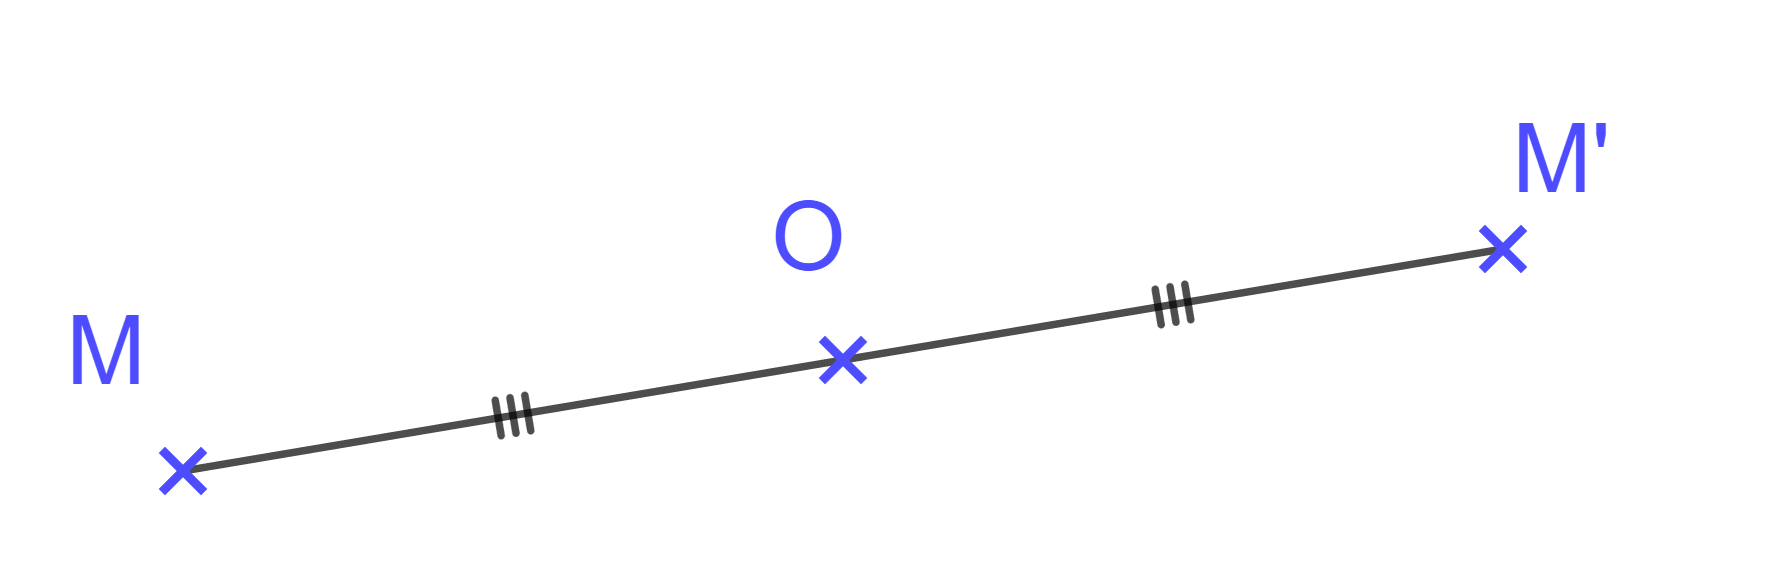
\includegraphics[scale=0.6]{img/fig3}
\end{center}

\label{LastPage}

%\section{Consommation électrique}
%
%Une consommation d'électricité se mesure en 
\end{document}